\subsection{Completed matched controls and actual catalog scaling}\label{sec:review-controls}
The completed review-control campaign comprises four exact public-center Full cases and ten plain/certified reuse cases. It audits MNIST catalogs of 64, 256 and 1,024 records and a 64-record CIFAR/ResNet catalog, each against ten approved public center sets. Learned/energy and PCA/energy use the same original integer rows, center sets, catalog root and task coverage as their exact control. The original rank-15 configurations use $T=4096$ and batch 64. Two predeclared MNIST $N=256$ pilots use rank 63, $T=16384$ and batch 16. All cases finish; no table infers proof completion from native execution or extrapolates unproved catalog batches.

Exact Full takes the full center coordinates as public inputs, authenticates original rows directly, and pays one compilation/setup for all ten sets. It needs no Stage~1. Under the common 1.6-million-constraint guard, Full uses batch eight for MNIST and two for CIFAR. Its four controls contain 80, 320, 1,280 and 320 actual proofs respectively. Every proof passes independent public-only replay, and local integer-reference analysis reproduces every saved Full label and aggregate cost (Table~\ref{tab:public-full-complete}). Different feasible batches are part of the measured resource-bounded configurations, rather than a claim that one batch is universally optimal.
\begin{table*}[tp]
\caption{Completed exact public-center Full controls. One setup serves all ten center sets; every catalog batch is proved and independently replayed. Peak RSS describes the prover process tree, excluding the Python driver. Component costs include native answer construction.}\label{tab:public-full-complete}
\centering\small
\begin{adjustbox}{max width=\textwidth}
\begin{tabular}{@{}llllll@{}}
\toprule
Catalog & Batch & Proofs & Constraints & Cost (s) & Peak RSS (GiB) \\
\midrule
CIFAR/ResNet $N=64$ & 2 & 320 & 1,061,820 & 5,351.1 & 2.19 \\
MNIST $N=64$ & 8 & 80 & 1,416,899 & 1,715.9 & 3.19 \\
MNIST $N=256$ & 8 & 320 & 1,422,913 & 6,237.9 & 3.21 \\
MNIST $N=1024$ & 8 & 1280 & 1,428,927 & 24,681.3 & 3.27 \\
\bottomrule
\end{tabular}
\end{adjustbox}
\end{table*}


For each deployment alternative, component cost includes native preparation, Stage~1 where applicable, query compilation/setup, native answer construction, witnesses and measured proving. Shared preprocessing is charged once; the exploratory plain-query phase is not charged to the certified alternative. Verification, warmups, fitting, I/O and public-center-statistic preparation are excluded and retained separately in the raw phase records. The first frozen Full worker omitted native answer construction from its CSV; we reconstruct that component from its saved samples without changing original results. All cases run serially on the same host, with one measured repetition per sample and one initial warmup. These totals measure a chosen deployment's components, not end-to-end online latency or timing variability across machines.

At $N=1024$, exact Full costs 24,681.3\,s, compared with 4,778.1\,s for plain learned reuse and 4,861.0\,s for certified learned reuse. The Full/component-cost ratios are 5.17 and 5.08. Main learned certified ratios range from 4.15 on MNIST $N=64$ to 8.07 on CIFAR $N=64$ (Table~\ref{tab:matched-public-full}). PCA/energy costs are similar: its $N=1024$ plain and certified totals are 4,823.8 and 4,904.6\,s. There is no general proof-speed advantage from selecting the learned basis instead of PCA at this representation width.
\begin{table*}[tp]
\caption{Completed matched audits over ten public center sets, rank 15 and $T=4096$. Each alternative pays preparation and setup once; every catalog row is proved. Component costs include native answer construction and exclude verification, fitting, warmups, I/O and public-center preparation. Full/certified compares different fidelity guarantees.}\label{tab:matched-public-full}
\centering\small
\begin{adjustbox}{max width=\textwidth}
\begin{tabular}{@{}lllllll@{}}
\toprule
Catalog & Method & Exact Full (s) & Plain (s) & Certified (s) & Full / certified & Cert. overhead (\%) \\
\midrule
CIFAR/ResNet $N=64$ & Learned + energy & 5,351.1 & 639.7 & 663.2 & 8.07 & 3.67 \\
CIFAR/ResNet $N=64$ & PCA + energy & 5,351.1 & 629.8 & 646.6 & 8.28 & 2.66 \\
MNIST $N=64$ & Learned + energy & 1,715.9 & 361.9 & 413.5 & 4.15 & 14.26 \\
MNIST $N=64$ & PCA + energy & 1,715.9 & 367.3 & 419.9 & 4.09 & 14.33 \\
MNIST $N=256$ & Learned + energy & 6,237.9 & 1,274.3 & 1,309.2 & 4.76 & 2.74 \\
MNIST $N=256$ & PCA + energy & 6,237.9 & 1,271.1 & 1,309.7 & 4.76 & 3.04 \\
MNIST $N=1024$ & Learned + energy & 24,681.3 & 4,778.1 & 4,861.0 & 5.08 & 1.74 \\
MNIST $N=1024$ & PCA + energy & 24,681.3 & 4,823.8 & 4,904.6 & 5.03 & 1.68 \\
\bottomrule
\end{tabular}
\end{adjustbox}
\end{table*}


The 1,024-record learned case replays 1,344 proofs: 1,024 Stage~1 proofs, 160 plain queries and 160 certified queries. Adding certification increases its query constraints from 616,148 to 740,617, but raises total component cost by only 1.74\% because preprocessing is shared. The corresponding PCA overhead is 1.68\%; at $N=64$, learned and PCA overheads are 14.26\% and 14.33\%. The largest exact Full process-tree RSS is 3.27\,GiB, versus 1.65\,GiB for the 1,024-record learned case; neither figure includes the Python driver or represents whole-host memory. Figure~\ref{fig:matched-scale} shows the measured scale result together with the difference between observed and certified accuracy.
\begin{figure*}[tp]
\centering
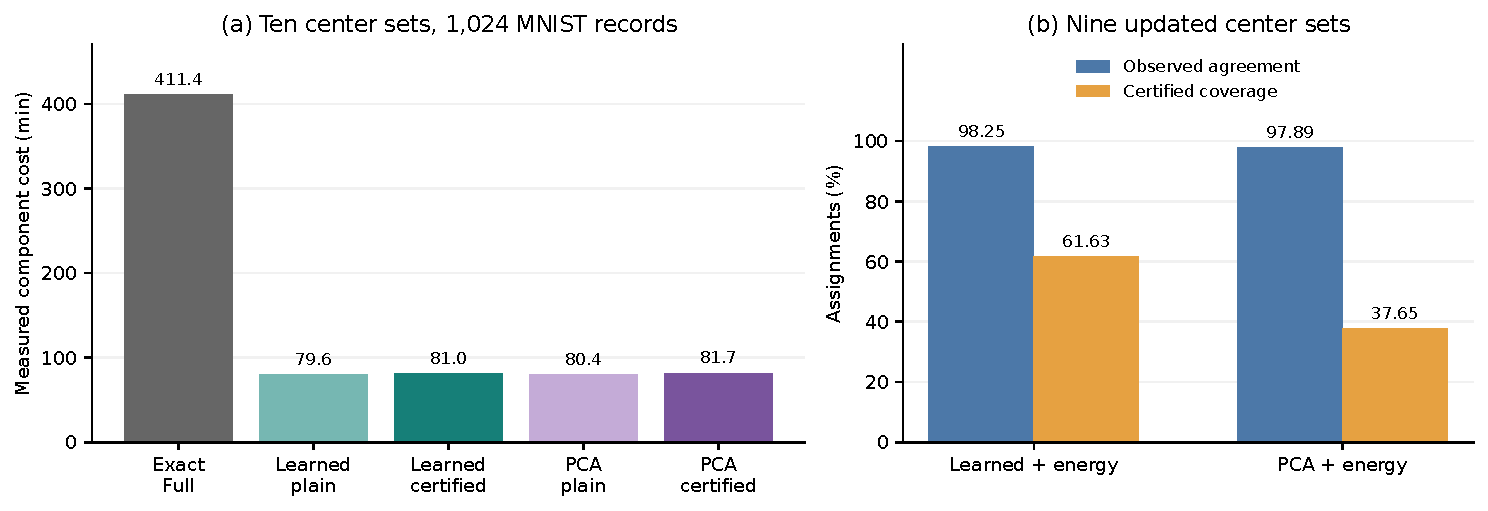
\includegraphics[width=\textwidth]{paper_results/review_controls/generated_completed_20261020/matched_scale.pdf}
\caption{Completed 1,024-record MNIST audit. (a) Measured component costs across ten public center sets, with setup and preprocessing charged once per alternative. Exact Full and approximate reuse provide different fidelity guarantees. (b) Mean agreement with quantized Full and guaranteed assignment coverage across nine updated sets. High empirical agreement does not imply that every assignment is certified.}
\label{fig:matched-scale}
\end{figure*}

\subsection{Proved accuracy envelopes and representation budgets}
The cost reductions come with a different verification contract. At $N=1024$, learned/energy agrees with quantized Full on 98.25\% of assignments on average across updated sets, while the proved correct-assignment count covers 61.63\% of rows on average and falls to 21.09\% for the worst update. Mean relative cost-interval width is 20.65\%. PCA gives 97.89\% agreement, 37.65\% coverage and 37.97\% width. Table~\ref{tab:matched-certificate-quality} reports all four main catalogs. Certified coverage is a lower bound for each individual set; an average across sets is descriptive and cannot replace its particular certificate.
\begin{table*}[tp]
\caption{Completed integer certificate quality at rank 15, $T=4096$. Agreement, certified coverage and relative cost-interval width are means across nine updated center sets. All checked intervals contain the exact quantized optimum; no certified assignment is incorrect.}\label{tab:matched-certificate-quality}
\centering\small
\begin{adjustbox}{max width=\textwidth}
\begin{tabular}{@{}llrrr@{}}
\toprule
Catalog & Method & Agreement (\%) & Certified (\%) & Width (\%) \\
\midrule
CIFAR/ResNet $N=64$ & Learned + energy & 99.48 & 60.76 & 24.00 \\
CIFAR/ResNet $N=64$ & PCA + energy & 98.44 & 39.76 & 33.58 \\
MNIST $N=1024$ & Learned + energy & 98.25 & 61.63 & 20.65 \\
MNIST $N=1024$ & PCA + energy & 97.89 & 37.65 & 37.97 \\
MNIST $N=256$ & Learned + energy & 98.31 & 59.20 & 20.51 \\
MNIST $N=256$ & PCA + energy & 97.44 & 35.98 & 38.10 \\
MNIST $N=64$ & Learned + energy & 98.26 & 52.26 & 20.80 \\
MNIST $N=64$ & PCA + energy & 96.53 & 30.03 & 38.19 \\
\bottomrule
\end{tabular}
\end{adjustbox}
\end{table*}


All 100 proved method/set outputs match the independent Python integer certificate, including assignment flags, count and both cost endpoints. Across 33,280 record/set evaluations, no certified assignment is incorrect and no interval misses the exact quantized optimum. These finite checks test implementation consistency; Proposition~\ref{prop:integer-envelope} supplies the general bound. The reported certified fractions and interval widths describe the guarantee available for each task without assigning a universal pass/fail threshold. The measured cost ratios do not establish equally exact services or authorize using small empirical point errors in place of the certificate.

The completed higher-rank proof pilots improve accuracy and certificate utility at increased component cost (Table~\ref{tab:proved-certificate-budget}). On MNIST $N=256$, learned rank-63/$T=16384$ gives 99.74\% agreement, 85.20\% certified coverage and 7.26\% mean width. Plain and certified totals are 1,731.2 and 1,834.8\,s, versus 1,274.3 and 1,309.2\,s at rank 15. PCA's higher-rank counterpart gives 99.70\% agreement, 80.51\% coverage and 8.88\% width. Both pilots replay all 576 proofs per case, including Stage~1. Rank, basis precision and query batch change together; these are combined configuration effects rather than an isolated causal effect of rank.
\begin{table*}[tp]
\caption{Completed predeclared MNIST $N=256$ rank-63, $T=16384$ proof pilots (batch 16). Quality means exclude the deployed set; costs cover all ten sets. Rank, precision and batching change together, so cost differences are configuration effects rather than an isolated rank ablation.}\label{tab:proved-certificate-budget}
\centering\small
\begin{adjustbox}{max width=\textwidth}
\begin{tabular}{@{}lllllll@{}}
\toprule
Method & Plain (s) & Certified (s) & Full / certified & Agreement (\%) & Certified (\%) & Width (\%) \\
\midrule
Learned + energy & 1,731.2 & 1,834.8 & 3.40 & 99.74 & 85.20 & 7.26 \\
PCA + energy & 1,753.5 & 1,850.1 & 3.37 & 99.70 & 80.51 & 8.88 \\
\bottomrule
\end{tabular}
\end{adjustbox}
\end{table*}


The native controls are retained separately in the artifact. The 1,024-record catalog extends the same held-out MNIST ordering; its first 256 quantized rows exactly match the earlier catalog. The deployed basis, scales, salts and ten center sets are retained without fitting on added audit rows. The original native preflight contains 80 method/set cells and 28,160 record/set evaluations; its rank-15 cases overlap the subsequently proved controls and are not independent observations.

A training-only native budget grid evaluates ranks 15/31/63/127 and basis scales 4096/16384 on the same 1,024 rows and ten sets. All cells are retained, and the rank-63 high-scale proof pilots were specified before inspecting these outcomes. Rank 15's high-scale control rescales the original rounded basis; larger ranks fit training data and round at each scale. At rank 63 and $T=16384$, learned/energy obtains 99.75\% agreement, 85.84\% mean coverage and 7.37\% width; rank 127 gives 90.32\% coverage and 4.64\% width. PCA also improves (Table~\ref{tab:native-certificate-budget}). These higher-rank 1,024-record cells are native calculations, not proof benchmarks; only the 256-record rank-63 configurations above have measured proof costs.
\begin{table*}[tp]
\caption{Native MNIST $N=1024$ budget controls (nine updated sets, quantized Full reference). All ranks and both basis scales are retained in the CSV artifact; this table shows the original configuration and larger-rank high-scale controls. These are not proof benchmarks.}\label{tab:native-certificate-budget}
\centering\small
\begin{adjustbox}{max width=\textwidth}
\begin{tabular}{@{}llrrrr@{}}
\toprule
Head rank / $T$ & Method & Agreement (\%) & Certified (\%) & Worst (\%) & Width (\%) \\
\midrule
15/4096 & Learned + energy & 98.25 & 61.63 & 21.09 & 20.65 \\
15/4096 & PCA + energy & 97.89 & 37.65 & 16.02 & 37.97 \\
31/16384 & Learned + energy & 99.36 & 76.86 & 31.05 & 12.28 \\
31/16384 & PCA + energy & 99.35 & 63.43 & 29.00 & 18.53 \\
63/16384 & Learned + energy & 99.75 & 85.84 & 45.80 & 7.37 \\
63/16384 & PCA + energy & 99.71 & 81.89 & 44.92 & 8.98 \\
127/16384 & Learned + energy & 99.86 & 90.32 & 59.86 & 4.64 \\
127/16384 & PCA + energy & 99.84 & 88.61 & 60.06 & 5.22 \\
\bottomrule
\end{tabular}
\end{adjustbox}
\end{table*}


Across the complete campaign, all 6,848 proofs pass independent public-only replay: 2,000 exact Full proofs and 4,848 Stage~1/plain/certified reuse proofs. Local analysis validates 208 captured metadata hashes, approved task coverage, matching original rows and centers, exact integer Full outputs and the independent certificate outputs. Targeted tests additionally reject altered roots, keys, indices, assignments and valid-range changes to certificate outputs. Optional tolerance-checker tests apply different user requirements to the same valid smoke certificate, separately from proof verification. The measurements themselves are reported as certified counts, cost intervals and observed agreement; application-specific tolerances are not treated as a benchmark success criterion.
